\chapter{Analogue Integrated Circuits}

\section{Differential Amplifier Circuit}

\begin{figure}[H]
  \centering
  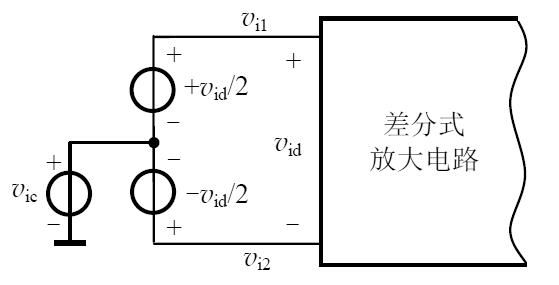
\includegraphics[width=0.5\linewidth]{figures/Differential-Amplifier}
\end{figure}

\begin{equation*}
  \begin{aligned}
    v_{i1} = v_{ic} + \dfrac{v_{id}}{2} \quad\quad
    v_{i2} = v_{ic} - \dfrac{v_{id}}{2} 
  \end{aligned}
\end{equation*}


\section{MOSFET Current Source}

\subsection{MOSFET Current Mirror}

\begin{figure}[H]
  \centering
  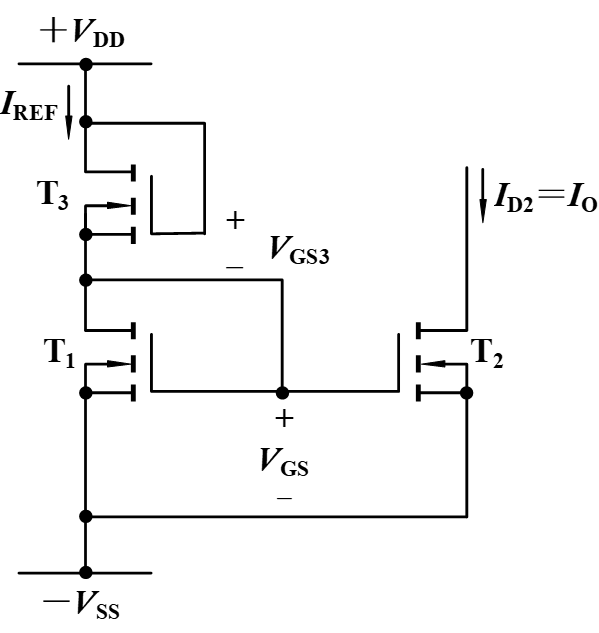
\includegraphics[width=0.4\linewidth]{figures/Current-Source}
\end{figure}

\begin{equation*}
  \begin{aligned}
    I_o = I_{D2} = K_n \left( V_{GS} - V_{TN} \right)^2
  \end{aligned}
\end{equation*}

\subsection{Cascade Current Mirror}

\begin{figure}[H]
  \centering
  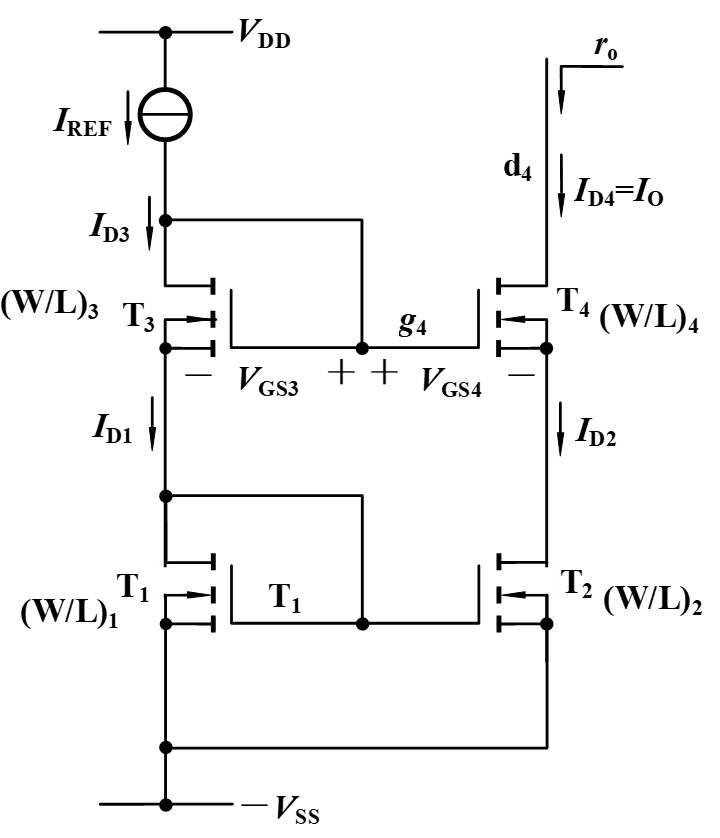
\includegraphics[width=0.5\linewidth]{figures/Cascade-Current-Source}
\end{figure}

The larger output resistance, the more stability of output current.

\begin{equation*}
  \begin{aligned}
    r_o = r_{ds4} + r_{ds2} \left( 1 + g_m r_{ds4} \right) \approx g_m r_{ds4} r_{ds2}
  \end{aligned}
\end{equation*}

\subsection{Combined Current Mirror}

\begin{figure}[H]
  \centering
  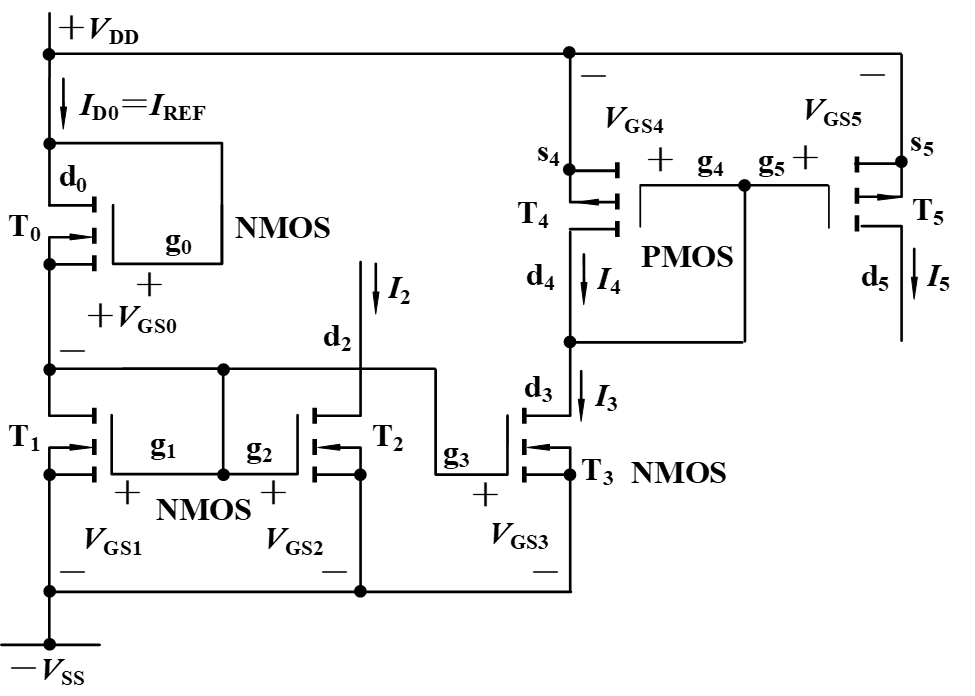
\includegraphics[width=0.6\linewidth]{figures/Combined-Current-Source}
\end{figure}

\begin{equation*}
  \begin{aligned}
    I_2 = \dfrac{\left( W / L \right)_2}{\left( W / L \right)_1} I_{REF} \quad\quad 
    I_3 = \dfrac{\left( W / L \right)_3}{\left( W / L \right)_1} I_{REF} \quad\quad 
    I_4 = I_3 \quad\quad 
    I_5 = \dfrac{\left( W / L \right)_5}{\left( W / L \right)_4} I_4
  \end{aligned}
\end{equation*}

\subsection{JFET Current Mirror}

\begin{figure}[H]
  \centering
  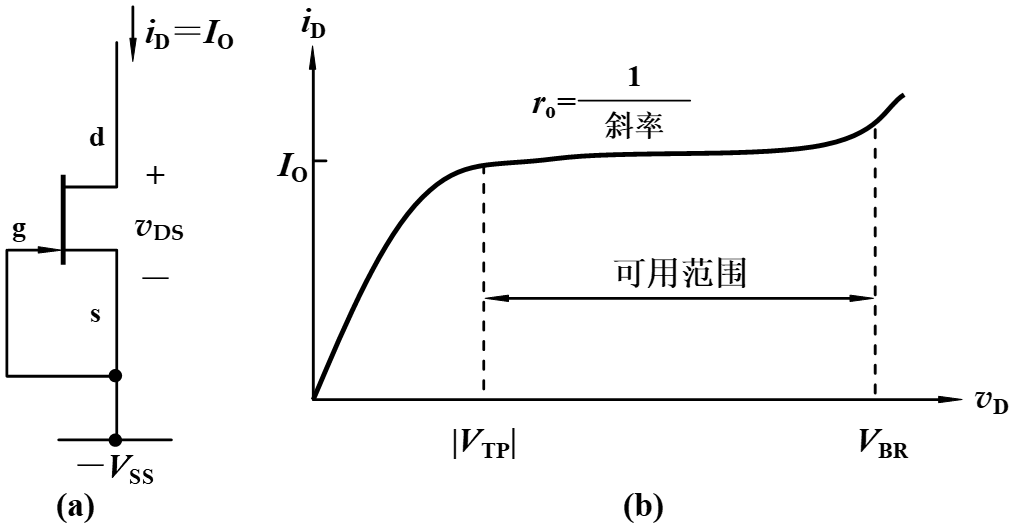
\includegraphics[width=0.9\linewidth]{figures/JFET-Current-Source}
\end{figure}

\begin{equation*}
  \begin{aligned}
    i_D = I_o = I_{DSS} \left( 1 + \lambda v_{DS} \right) \quad\quad 
    r_o = \dfrac{1}{\lambda I_{DSS}} 
  \end{aligned}
\end{equation*}

\section{BJT Current Source}

\subsection{BJT Current Mirror}

\begin{figure}[H]
  \centering
  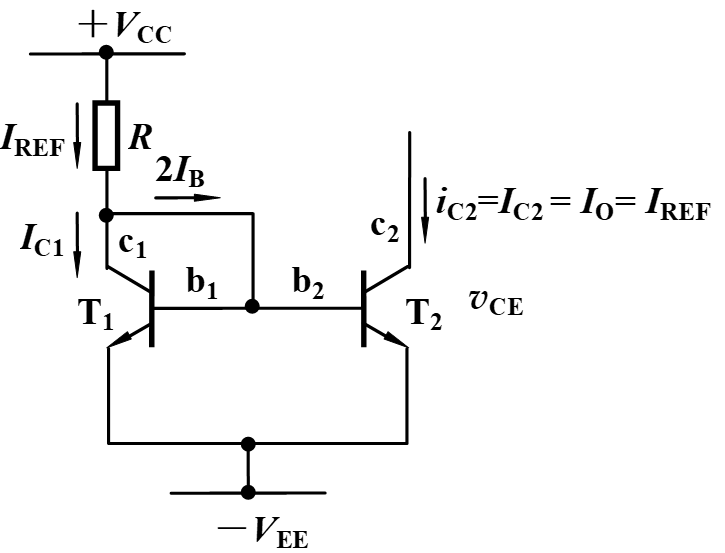
\includegraphics[width=0.7\linewidth]{figures/BJT-Current-Source}
\end{figure}

\begin{equation*}
  \begin{aligned}
    I_{C2} = I_{C1} \approx I_{REF} \approx \dfrac{V_{CC}}{R} 
    \quad\quad 
    r_o = r_{ce}
  \end{aligned}
\end{equation*}

\subsection{Micro Current Source}

\begin{figure}[H]
  \centering
  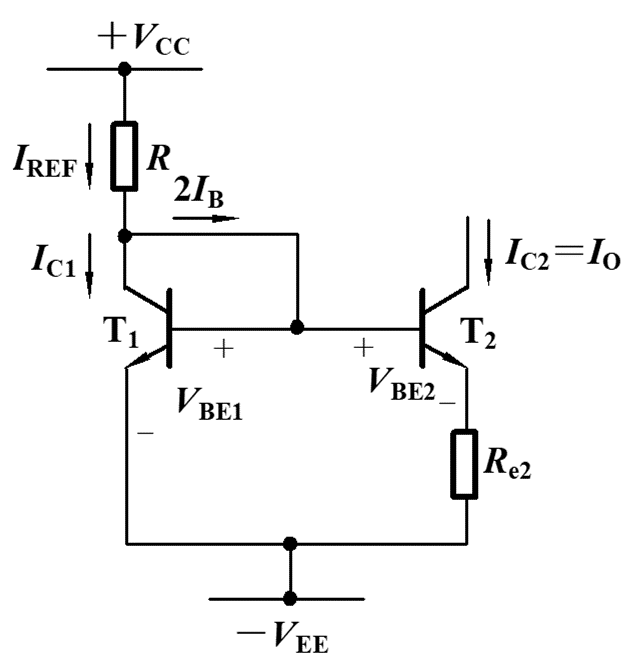
\includegraphics[width=0.6\linewidth]{figures/Micro-Current-Source}
\end{figure}

\begin{equation*}
  \begin{aligned}
    I_o = \dfrac{\Delta V_{BE}}{R_{e2}} \quad\quad 
    r_o \approx r_{ce2} + \left( 1 + \dfrac{\beta R_{e2}}{r_{be2} + R_{e2}}  \right)
  \end{aligned}
\end{equation*}

\subsection{Current Source with High Output Resistance}

\begin{figure}[H]
  \centering
  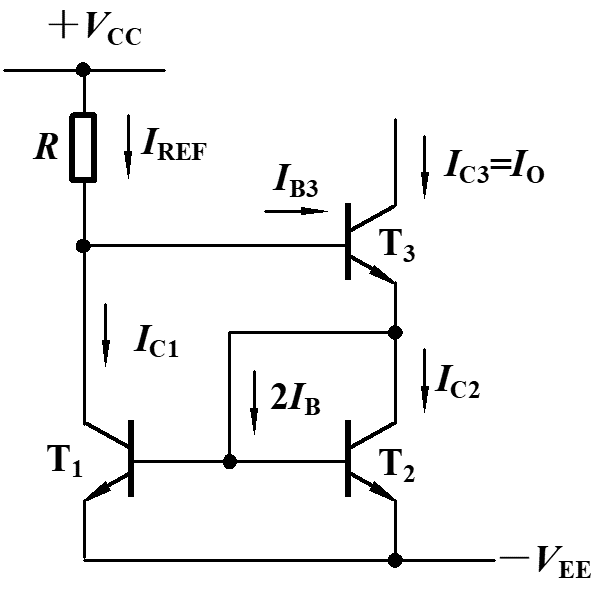
\includegraphics[width=0.5\linewidth]{figures/High-Resistance-Current-Source}
\end{figure}

\begin{equation*}
  \begin{aligned}
    I_{REF} = \dfrac{V_{CC} - V_{BE3} - V_{BE2} + V_{EE}}{R} \quad\quad 
    I_o \approx I_{C2} = \dfrac{A_3}{A_1} \cdot I_{REF} 
  \end{aligned}
\end{equation*}

\subsection{Combined Current Source}

\begin{figure}[H]
  \centering
  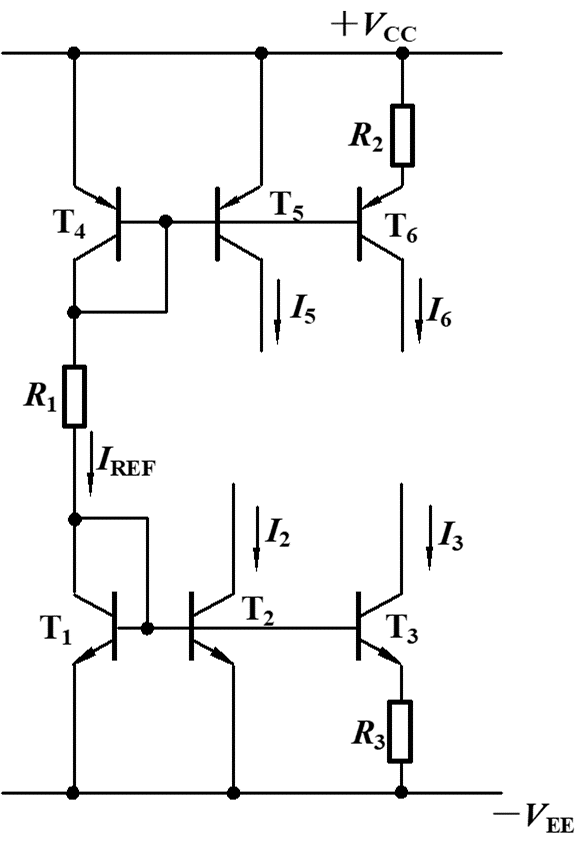
\includegraphics[width=0.4\linewidth]{figures/BJT-Combined-Current-Source}
\end{figure}

\begin{equation*}
  \begin{aligned}
    I_{REF} = \dfrac{V_{CC} + V_{EE} - V_{BE1} + V_{EB4}}{R_1} 
  \end{aligned}
\end{equation*}

\section{Differential Amplifier}

\subsection{MOSFET}

\subsubsection{Two Output Terminals}

\begin{figure}[H]
  \centering
    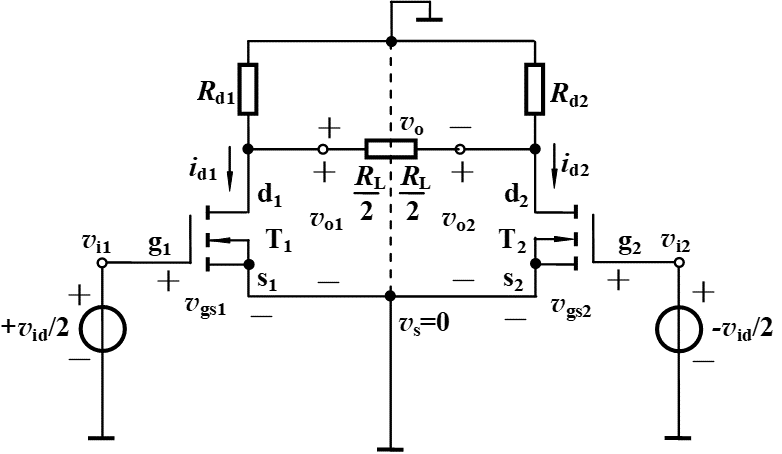
\includegraphics[width=0.7\linewidth]{figures/Differential-Amplifier-MOS-1}
\end{figure}

\begin{equation*}
  \begin{aligned}
    i_{d1} = i_{d2} = I_D = \dfrac{1}{2} I_o \quad\quad g_m = \sqrt{2 K_n I_o} \quad\quad A_{vd} = - g_m \left( r_{ds} \parallel R_d \parallel \dfrac{R_L}{2}  \right) \quad\quad K_{CMR} = \infty \quad\quad R_o = 2 R_d
  \end{aligned}
\end{equation*}

\subsubsection{One Output Terminal}

\begin{figure}[H]
  \centering
    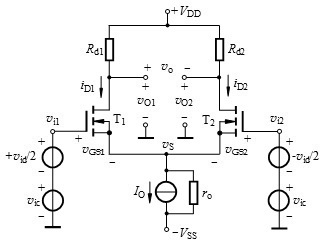
\includegraphics[width=0.7\linewidth]{figures/Differential-Amplifier-MOS-2}
\end{figure}

\begin{equation*}
  \begin{aligned}
    g_m = \sqrt{2 K_n I_o} \quad\quad A_{vd1} = - A_{vd2} = - \dfrac{g_m \left( r_{ds} \parallel R_d \parallel R_L \right) }{2} \quad\quad K_{CMR} \approx g_m r_o \quad\quad R_o = R_d
  \end{aligned}
\end{equation*}

\subsection{BJT}

\subsubsection{Two Output Terminals}

\begin{figure}[H]
  \centering
  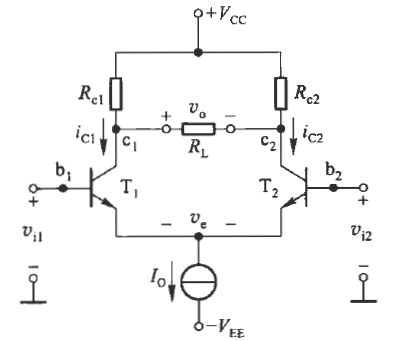
\includegraphics[width=0.7\linewidth]{figures/Differential-Amplifier-BJT-1}
\end{figure}

\begin{equation*}
  \begin{aligned}
    A_{vd} = - \dfrac{\beta \left( R_c \parallel \dfrac{R_L}{2} \right)}{r_{be}} \quad\quad K_{CMR} = \infty \quad\quad R_{id} = 2 r_{be} \quad\quad R_{ic} = \dfrac{1}{2} \left[ r_{be} + \left( 1 + \beta \right) 2 r_o \right] \quad\quad R_o = 2 R_c
  \end{aligned}
\end{equation*}

\subsubsection{One Output Terminal}

\begin{figure}[H]
  \centering
  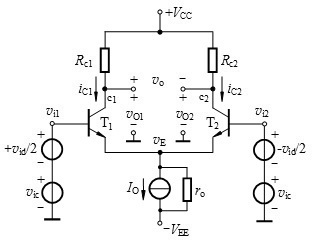
\includegraphics[width=0.7\linewidth]{figures/Differential-Amplifier-BJT-2}
\end{figure}

\begin{equation*}
  \begin{aligned}
    A_{vd1} = - A_{vd2} = - \dfrac{\beta \left( R_c \parallel R_L \right)}{2 r_{be}} \quad\quad K_{CMR} \approx \dfrac{\beta r_o}{r_{be}} \quad\quad R_{id} = 2 r_{be} \quad\quad R_{ic} = \dfrac{1}{2} \left[ r_{be} + \left( 1 + \beta \right) 2 r_o \right] \quad\quad R_o = R_c
  \end{aligned}
\end{equation*}

%%% Local Variables:
%%% mode: latex
%%% TeX-master: "Analogue_Electronics"
%%% End:
